%\chapterimage{Geometrijska.jpg} % Chapter heading image

\chapter{Interferenca}
\label{chap:Interferenca}
Spoznali bomo, da sta uklon in interferenca tesno povezana in pravzaprav
manifestacija istega pojava -- seštevanja  valovanj v 
skupno optično polje. V poglavju o uklonu so nas zanimali predvsem uklonski 
vzorci, v poglavju o interferenci pa se bomo osredotočili na interferometrijo 
in pojave na tankih plasteh.

\section{Interferenca in interferometrija}
O interferenci govorimo, kadar je na danem mestu v 
prostoru jakost električnega polja sestavljena iz 
več valovanj. Seštevanje 
dveh ali več valovanj ponekod vodi
do ojačevanja svetlobe (konstruktivna interferenca), 
drugod pa do oslabitev (destruktivna interferenca). 
Vzorci izmenjujočih se ojačitev in oslabitev sestavljajo
značilno interferenčno sliko.

Elektromagnetna valovanja se na splošno razlikujejo 
v smeri širjenja, amplitudi, frekvenci, fazi ali polarizaciji. 
Spoznali bomo, da se interferenčna slika pojavi le pri valovanjih z enako
polarizacijo, konstantno (ali zelo počasi se spreminjajočo)
začetno fazo in enako (oziroma približno enako) frekvenco. 
Če se frekvenci valovanj ne ujemata, se svetlobno valovanje na 
danem mestu zelo hitro spreminja in slika, ki jo zaznamo, se izpovpreči.
Zahteva o konstantni fazi je povezana s koherenco valovanja, 
ki jo bomo podrobneje obravnavali v poglavju~\ref{chap:Koherenca}. 

Najpreprostejši interferenčni poskusi so taki, pri katerih vpadni snop svetlobe
razdelimo na več delov. To lahko naredimo z delitvijo po valovni fronti
ali z delitvijo po amplitudi. V obeh primerih so zahteve po isti frekvenci, 
polarizaciji in začetni fazi izpolnjene, seveda pa se valovanji razlikujeta 
v dodatnem faznem zamiku, ki ga pridobita po delitvi.
Dodatni fazni zamik in z njim povezana interferenčna slika 
sta močno odvisna od dolžine poti, ki jo prepotuje del prvotnega snopa 
vpadne svetlobe. Ker je valovna dolžina svetlobe zelo majhna, že majhne 
spremembe v dolžini poti oziroma zakasnitvi žarka povzročijo velike spremembe 
interferenčnega vzorca. 

Z opazovanjem interferenčnih vzorcev lahko zelo natančno določimo fazni zamik med
dvema deloma valovanja in s tem pridobimo podatke o valovanju samem, o snovi, po 
kateri se širi valovanje, ali o oddaljenosti predmeta, od katerega se svetloba odbija. 
Zato interferometrijo, kot imenujemo metodo, ki temelji na opazovanju interference,
s pridom uporabljamo med drugim za izredno natančne meritve dolžine, 
oddaljenosti, lomnega količnika snovi oziroma njegovih sprememb ali odstopanj v frekvenci. 
Interferenčne meritve so ene najnatančnejših in so zato zelo uporabne na veliko področjih:
od prvotne opustitve obstanka etra prek izredno natančnih meritev gladkosti površine do
opazovanja gravitacijskih valov. 

V laboratorijih in industrijskih aplikacijah navadno za vir svetlobe uporabljamo laser, zato
je interferenčna slika sestavljena iz svetlih in temnih območij. V naravi interferenco
navadno opazujemo z belo dnevno svetlobo, kar da tankim plastem, na primer plasti olja na vodi ali
milnemu mehurčku, značilno mavrično obarvanost.

\section{Interferenca dveh ravnih valov}
Zapišimo preprost primer interference dveh ravnih valov z enako frekvenco. Valovna
vektorja valovanj označimo s $\mathbf{k}_1$ in $\mathbf{k}_2$, fazi valovanj z 
$\delta_1$ in $\delta_2$ ter njuni realni amplitudi z $E_{10}$ in $E_{20}$. Ker imajo 
valovanja, ki interferirajo, isto polarizacijo,
za račun interference zadošča skalarna oblika električnega polja.
Valovanji potem zapišemo kot:
\beq
E_1 = E_{10} e^{i\mathbf{k}_1 \cdot \mathbf{r} - i \omega t + i \delta_1}
\qquad \mathrm{in} \qquad
E_2 = E_{20} e^{i\mathbf{k}_2 \cdot \mathbf{r} - i \omega t + i \delta_2}.
\label{eq:06_01}
\eeq
Celotno
električno polje je vsota obeh prispevkov:
\beq
E = E_1 + E_2 = E_{10} e^{i\phi_1 - i \omega t} + E_{20} e^{i\phi_2 - i \omega t},
\label{eq:06_02}
\eeq
pri čemer sta $\phi_{1,2} = \mathbf{k}_{1,2} \cdot \mathbf{r} + \delta_{1,2}$. 
Gostota svetlobnega toka $j$ je na splošno (enačba~\ref{eq:j}):
\beq
j = \frac{1}{2}\varepsilon \varepsilon_0 |E|^2c,
\label{eq:06_03}
\eeq
zato je celotna gostota svetlobnega toka enaka:
\beq
j \propto (E_1+E_2)(E_1^*+E_2^*)  = 
\left( E_{10} e^{i\phi_1 - i \omega t} + E_{20} e^{i\phi_2 - i \omega t}\right)
\left( E_{10} e^{-i\phi_1 + i \omega t} + E_{20} e^{-i\phi_2 + i \omega t}\right)\!.
\label{eq:06_04}
\eeq
Sledi:
\beq
j \propto E_{10}^2 + E_{20}^2 + E_{10}E_{20} \left(e^{i\phi_1-i\phi_2}+ e^{-i\phi_1+i\phi_2}\right)\!.
\label{eq:06_05}
\eeq
Eksponente v oklepaju izrazimo s kotno funkcijo in upoštevajoč zvezo~(enačba~\ref{eq:06_03}) dobimo:
\boxeq{eq:06_06}{
j = j_1 + j_2 + 2\sqrt{j_1 j_2} \cos(\Delta \phi),
}
pri čemer sta $j_1$ in $j_2$ gostoti svetlobnih tokov prvega in drugega delnega valovanja,
$\Delta \phi$ pa označuje razliko faz $\phi_1-\phi_2$. Le kadar je ta razlika neodvisna
od časa oziroma se s časom zelo počasi spreminja, v eksperimentu poleg prvih dveh členov
v enačbi~(\ref{eq:06_06}) opazimo tudi tretjega. V nasprotnem primeru se tretji člen 
izpovpreči in intenziteta na opazovalnem zaslonu je enaka vsoti intenzitet posameznih 
delnih valovanj. Interference v tem primeru ne vidimo. 

Če je $\Delta \phi$ neodvisen od časa, gostota svetlobnega toka na opazovalnem zaslonu $j$
zavzema vrednosti $j_\mathrm{min}<j<j_\mathrm{max}$, za katere velja:
\beq
\left(j_1+j_2 -2\sqrt{j_1 j_2}\right) < j < \left(j_1+j_2 -2\sqrt{j_1 j_2}\right)
\label{eq:06_07}
\eeq
oziroma zapisano drugače:
\beq
\left(\sqrt{j_1}- \sqrt{j_2}\right)^2 < j < \left(\sqrt{j_1} +\sqrt{j_2}\right)^2\!\!.
\label{eq:06_07a}
\eeq
\begin{remark}
Vpeljemo lahko tudi kontrast interferenčnega vzorca, ki ga izračunamo kot:
\beq
v = \frac{j_\mathrm{max}- j_\mathrm{min}}{j_\mathrm{max}+ j_\mathrm{min}}.
\label{eq:06_08}
\eeq
Parameter $v$, ki zavzema vrednosti med 0 in 1, imenujemo tudi
vidljivost interferenčnega vzorca.
\end{remark}

Vrnimo se h krajevni odvisnosti gostote svetlobnega toka (enačba~\ref{eq:06_06}). Na
splošno se intenziteti delnih valovanj razlikujeta in skupna gostota svetlobnega
toka oscilira med neko neničelno najmanjšo in največjo vrednostjo (slika~\ref{fig:06_kontrast}).
\begin{figure}[h!]
\centering
\def\svgwidth{85truemm} 
\input{slike/06_vidljivost.pdf_tex}
\vglue1truemm
\caption{Interferenca dveh valovanj z različnima intenzitetama. 
Vrednost skupne gostote svetlobnega toka v odvisnosti od faznega 
zamika med vpadnima valovanjema oscilira med najmanjšo $j_\mathrm{min}$ 
in največjo vrednostjo $j_\mathrm{max}$. Pikčasta črta označuje skupno
gostoto toka delnih valovanj, kadar se fazna razlika hitro spreminja
in interferenčni vzorec ni viden.}
\label{fig:06_kontrast}
\end{figure}

V posebnem primeru, ko sta amplitudi obeh valovanj enaki in je $j_1 = j_2 = j_0$, 
je skupna gostota svetlobnega toka enaka (enačba~\ref{eq:06_06}):
\beq
j = 2j_0 + 2j_0 \cos (\Delta \phi) = 4j_0 \cos^2 (\Delta \phi/2).
\label{eq:06_09}
\eeq
Interferenčni vzorec dveh enako močnih snopov svetlobe zavzema vrednosti med 0 
in $4j_0$, kar pomeni, da je kontrast takega vzorca (enačba~\ref{eq:06_08}) enak 1. 
Kadar se fazna razlika med valovanjema $\Delta \phi$ hitro spreminja,
je gostota svetlobnega toka na zaslonu enaka vsoti prispevkov posameznih 
delnih valovanj in interference ne vidimo. Takrat je kontrast enak 0. 

Kako pa je z ohranitvijo energijskega toka pri interferenci? Omejimo 
se na primer, ko sta amplitudi obeh delnih valovanj enaki. Takrat
je povprečni energijski  tok čez veliko območje prostora enak (enačba~\ref{eq:06_09}):
\beq
\langle j \rangle = \langle 4j_0 \cos^2 (\Delta \phi/2) \rangle  = \frac{1}{2}(4j_0) = 2j_0.
\label{eq:06_10}
\eeq
Po pričakovanju je povprečna gostota energijskega toka interferenčnega vzorca
enaka vsoti gostot energijskega toka obeh vpadnih valovanj. Enako velja tudi 
v primeru, ko amplitudi vpadnih delnih valovanj nista enaki. Pri interferenci se 
torej energijski tok ohranja, vendar se energija prerazporedi.

\begin{example}{\bf Interferenca dveh ravnih valovanj.}
Opazujmo interferenco dveh ravnih valovanj z enakima intenzitetama, ki pod kotom 
vpadata eno glede na drugo (slika~\ref{fig:06_int}). Njuna valovna vektorja na splošno
zapišemo kot: $\mathbf{k}_1 = (k_x,0, k_z)$ in $\mathbf{k}_2 = (-k_x,0, k_z)$. 
Valovanji sta oblike:
\beq
E_1 = E_0 e^{ik_x x} e^{ik_z z}e^{-i\omega t} \qquad \mathrm{in} \qquad 
E_2 = E_0 e^{-ik_x x} e^{ik_z z}e^{-i\omega t}.
\label{eq:06_12}
\eeq
Interferenca teh dveh valovanj da:
\beq
E = E_1+E_2 = E_0 e^{ik_z z -i\omega t }\left(e^{ik_x x}+e^{-ik_x x} \right) = 
E_0 e^{ik_z z -i\omega t } 2 \cos(k_x x).
\label{eq:06_14}
\eeq
Izračunamo gostoto svetlobnega toka in za interferenčni vzorec dobimo obliko:
\beq
j = 4 j_0 \cos^2(k_x x).
\label{eq:06_15}
\eeq
\begin{figure}[!h]
\centering
\def\svgwidth{120truemm} 
\input{slike/06_interferenca_1.pdf_tex}
\caption{Interferenca dveh ravnih valovanj, ki pod kotom vpadata eno na drugo. 
Prikaz električne poljske jakosti (a) in intenzitete (b). 
Modra barva označuje negativno vrednost jakosti električnega polja in 
rdeča pozitivno. Kjer je belo, je jakost električnega polja enaka nič.
Intenzitetni interferenčni vzorec (b)
ima značilne bele črte na mestu oslabitev, potujoče ojačitve z leve slike pa se 
na detektorju izpovprečijo v znano interferenčno sliko.}
\label{fig:06_int}
\end{figure}

\end{example}

\begin{example}{\bf Interferenca dveh krožnih valovanj.}
Poglejmo še interferenco dveh krožnih valovanj v ravnini. Krožno valovanje izhaja
iz ene točke in se v koncentričnih krogih širi po ravnini navzven. V
ravnini $xy$ dve krožni valovanji zapišemo kot:
\beq
E_1 \propto \exp\left( ik\sqrt{x^2+y^2}\right)  e^{-i\omega t}
\qquad \mathrm{in} \qquad
E_2 \propto \exp\left( ik\sqrt{(x-d)^2+y^2}\right)  e^{-i\omega t}.
\label{eq:06_16a}
\eeq
Pri zapisu smo privzeli, da sta izhodišči valovanj razmaknjeni vzdolž osi $x$, 
razmik med njima pa je enak $d$. Pojemanja amplitude
z oddaljenostjo od izvora nismo zapisali. Nekaj primerov amplitudnih in pripadajočih
intenzitetnih interferenčnih vzorcev, ki 
nastanejo pri različnih razmikih $d$ in različni valovni dolžini, 
je narisanih na sliki~\ref{fig:06_intkrog}.
\begin{figure}[!h]
\centering
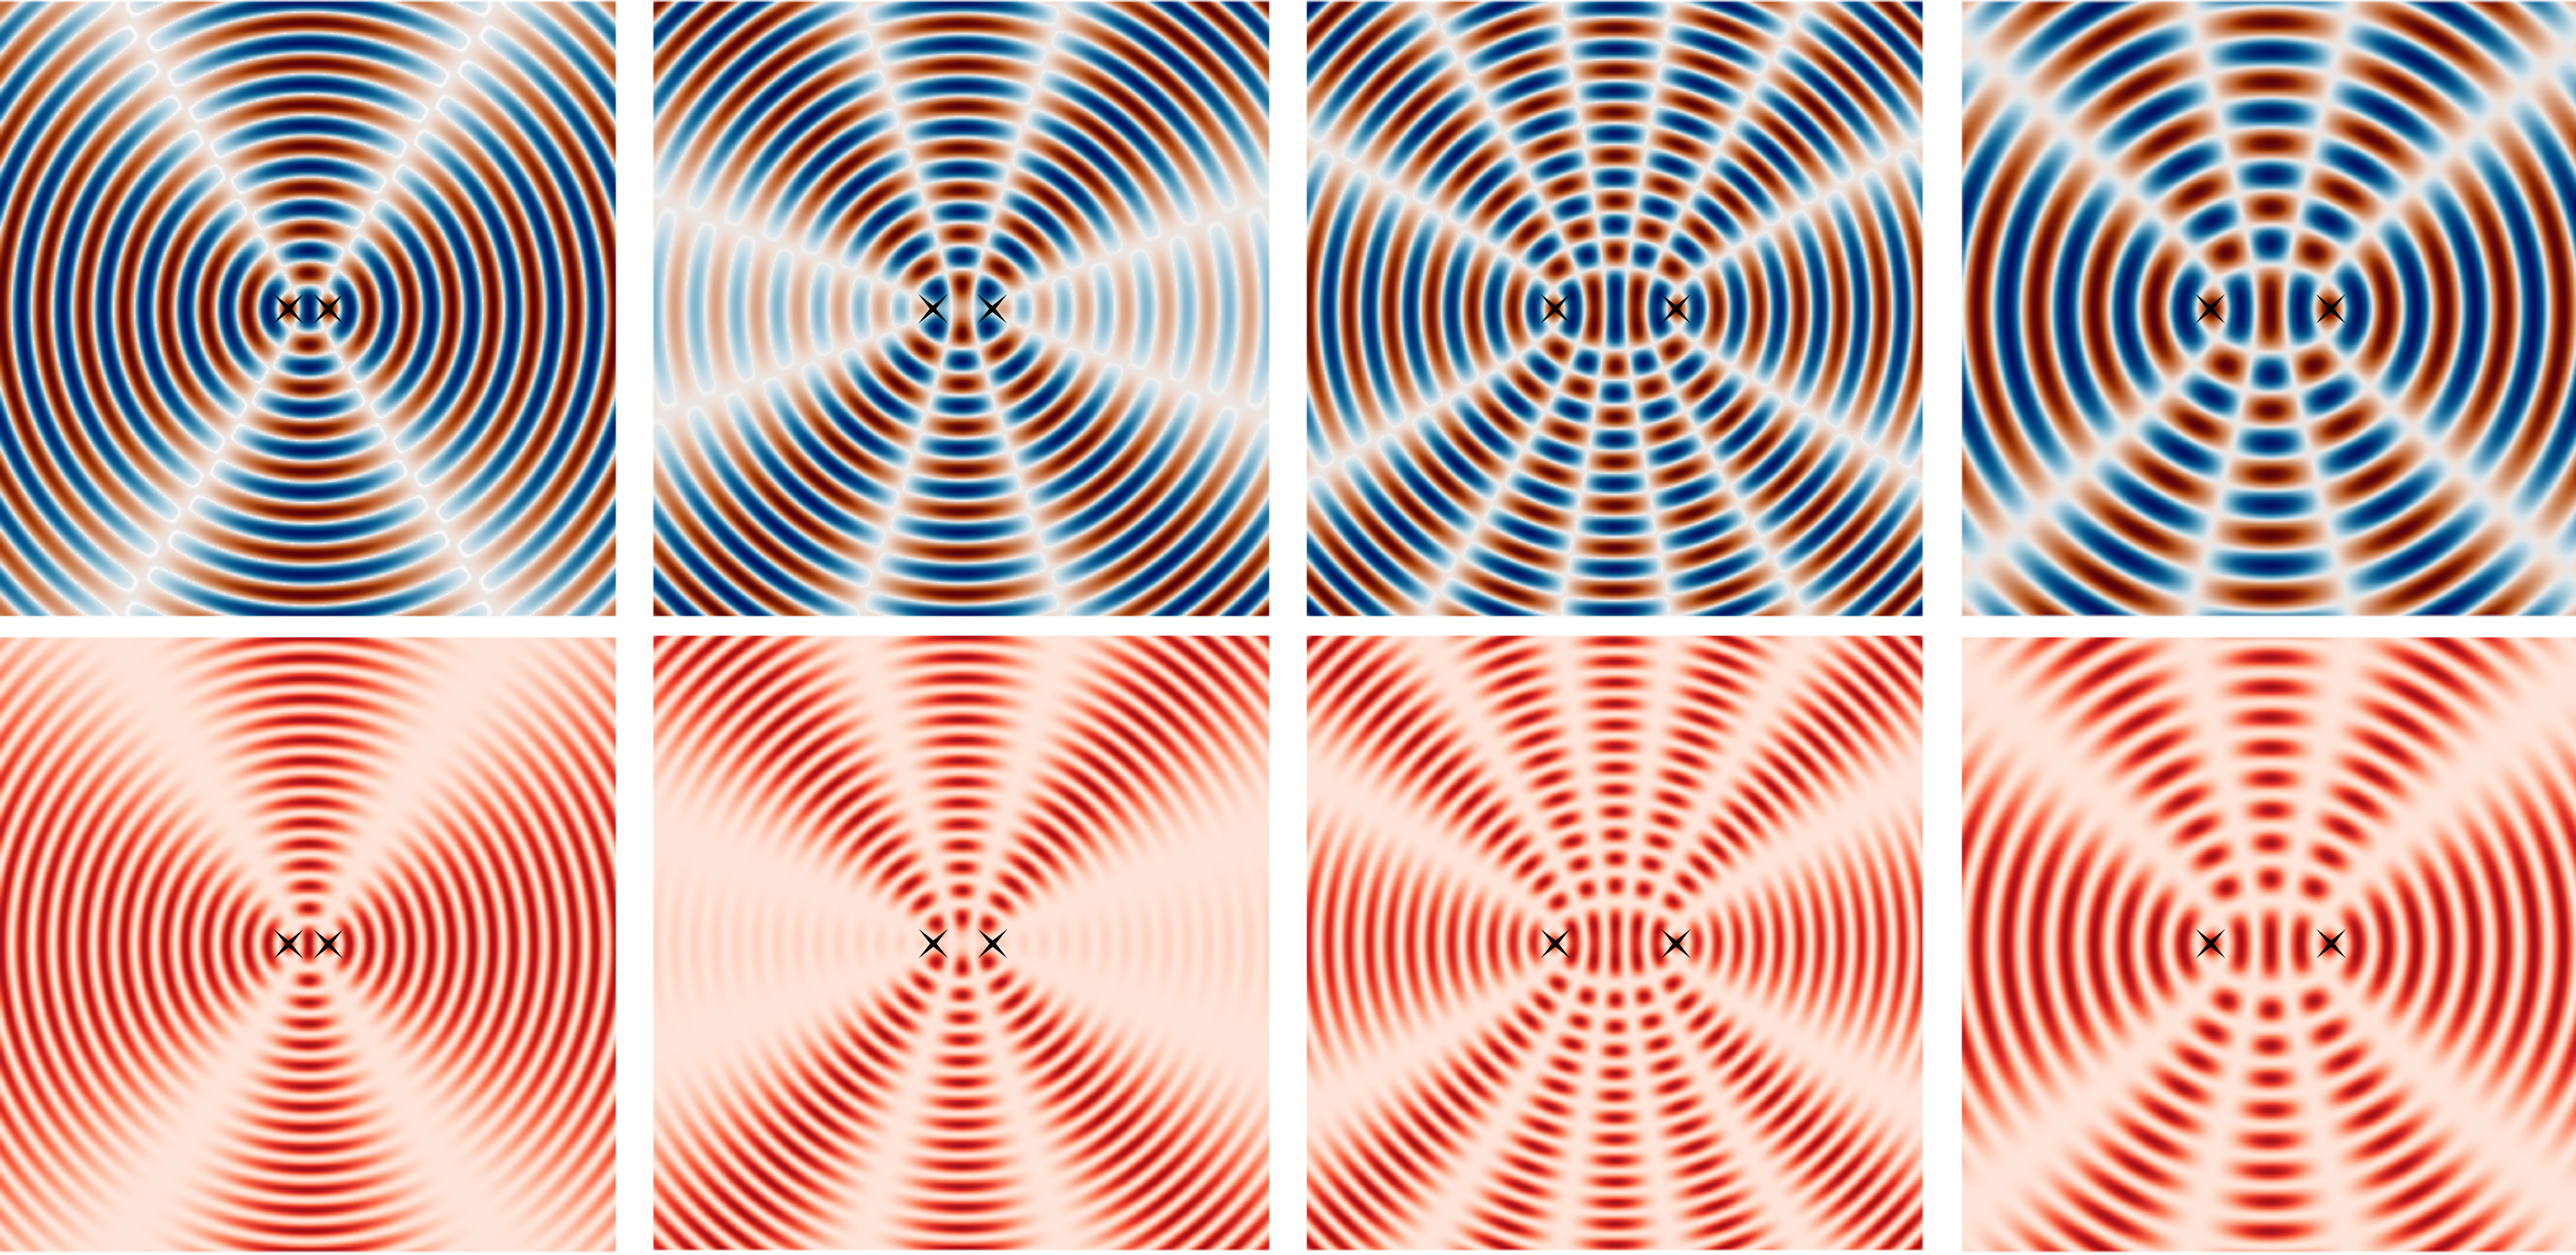
\includegraphics[width=140truemm]{slike/06_interferenca_krog_nov.png}
\caption{Interferenca dveh krožnih valov, pri čemer zgornja vrsta prikazuje 
amplitudo polja, spodnja pa intenziteto. Na mestih, kjer sta valovanji iz faze (destruktivna
interferenca), se pojavijo oslabitve, kjer sta valovanji v fazi (konstruktivna interferenca),
pa ojačitve. Od leve proti desni razmik med izvoroma narašča, zato se ojačitve gostijo, zadnji 
stolpec pa ponazori premik ojačitev pri spremenjeni valovni dolžini valovanja.}
\label{fig:06_intkrog}
\vglue-5truemm
\end{figure}

\end{example}

\section{Interferenca z delitvijo valovne fronte}
Pri večini interferenčnih poskusov ustvarimo interferenco z enim samim 
snopom svetlobe, ki ga razdelimo na dva dela. S tem zagotovimo isto 
frekvenco, isto začetno fazo in enako polarizacijo obeh delnih valovanj. V uvodu smo
že omenili, da lahko vpadno valovanje razdelimo na dva dela z delitvijo 
valovne fronte valovanja (npr. Youngov poskus) ali z delitvijo amplitude
valovanja (npr. Michelsonov interferometer). Najprej si poglejmo prvi primer.

Najpomembnejši primer interference z delitvijo valovne fronte je nedvomno
Youngov poskus (1801), na podlagi katerega je angleški fizik Thomas Young
sklepal, da je svetloba transverzalno valovanje. 
Pri tem poskusu vpadno valovanje iz monokromatskega izvora  
simetrično usmerimo na objektni zaslon, v katerem sta dve enaki ozki
reži, in opazujemo sliko na oddaljenem zaslonu\footnote{Vpadno valovanje mora biti 
kar se da koherentno. Young je to dosegel tako, da je vpadno svetlobo najprej 
speljal skozi eno tanko režo in jo šele nato usmeril na zaslon z dvema režama. 
Več o koherenci bomo spoznali v poglavju~\ref{chap:Koherenca}.}. Poiščimo 
lego ojačitev in oslabitev na oddaljenem opazovalnem zaslonu.
\begin{figure}[ht]
\centering
\def\svgwidth{100truemm} 
\input{slike/06_Young.pdf_tex}
\caption{Pri prvotnem Youngovem poskusu monokromatska svetloba prehaja ozko 
režo in vpada simetrično na dve ozki reži v razmiku $D$ na objektnem zaslonu. 
Na oddaljenem zaslonu opazujemo interferenčno sliko. Pri tem $z_0$ opisuje razdaljo
od objektnega do opazovalnega zaslona, $r_1$ in 
$r_2$ razdalji od rež do izbrane točke na opazovalnem zaslonu in kot 
$\vartheta$ približno smer izbrane točke glede na reži v zaslonu. 
Privzamemo, da je $z_0 \gg D$.}
\label{fig:06_Young}
\vglue-3truemm
\end{figure}

Naj bodo $z_0$ razdalja od objektnega zaslona z dvema režama 
do opazovalnega zaslona, $D$ razdalja med središčema rež, 
$r_1$ razdalja med sredino prve reže in izbrano točko na zaslonu
ter $r_2$ razdalja med sredino druge reže in isto točko na zaslonu. Potem za velike 
oddaljenosti $r_1, r_2 \gg D$ velja:
\beq
\Delta r = r_1-r_2 \approx D \sin\vartheta,
\label{eq:06_16}
\eeq
pri čemer je $\vartheta$ kot med osjo $z$ in zveznico med točko na sredini med režama in
izbrano točko na opazovalnem zaslonu. Ker ležita reži simetrično, sta intenziteti delnih
valovanj enaki, prav tako tudi njuni začetni fazi. Za izračun gostote svetlobnega toka na zaslonu 
zato lahko uporabimo enačbo~(\ref{eq:06_09}). Vstavimo fazno razliko $\Delta \phi \approx 
k\Delta r$ in z upoštevanjem enačbe~(\ref{eq:06_16}) dobimo:
\beq
j = 4 j_0 \cos^2\left(\frac{\Delta \phi}{2}\right) = 4j_0 \cos^2\left(\frac{k\Delta r}{2}\right) = 
4j_0 \cos^2\left(\frac{kD\sin \vartheta}{2}\right)\!\!.
\label{eq:06_17}
\eeq
V točkah, kjer se prispevka obeh valovanj seštejeta, nastopi 
konstruktivna interferenca in na zaslonu opazimo ojačitve. 
Izhajajoč iz enačbe~(\ref{eq:06_17}) pogoj za ojačitev zapišemo kot:
\beq
\frac{kD\sin \vartheta}{2} = N\pi,
\label{eq:06_18}
\eeq
pri čemer je $N$ celo število. 

Od tod izračunamo pogoj za kote $\vartheta_\mathrm{max}$, pri katerih
se pojavijo ojačitve:
\boxeq{eq:InterferencaMax}{
D \sin\vartheta_\mathrm{max} = N \lambda.
}
Zapis pove, da se ojačitve pojavijo, ko je razlika poti od rež 
do točke na zaslonu enaka večkratniku valovne dolžine valovanja.

V vmesnih točkah, kjer se prispevka valovanj odštejeta, nastopi 
destruktivna interferenca in na zaslonu opazimo oslabitve (neosvetljene proge). 
Pogoj za oslabitve je:
\boxeq{eq:InterferencaMin}{
D \sin\vartheta_\mathrm{min} = \left(N + \frac{1}{2}\right)\lambda.
}
Interferenčni vzorec, ki ga opazujemo na oddaljenem opazovalnem zaslonu, je za majhne 
kote periodičen. Izračunajmo periodo ponavljanja $\xi_0$ (slika~\ref{fig:06_Young}). 
Iz enačbe~(\ref{eq:06_17}) sledi zahteva:
\beq
\Delta \left(\frac{kD\sin \vartheta}{2}\right) = \pi.
\label{eq:06_19}
\eeq
Za majhne kote velja $\sin \vartheta \approx \vartheta$ in zapišemo: 
\beq
\frac{k D\,\Delta \sin\vartheta}{2} \approx \frac{k D\, \Delta \vartheta}{2}
 \approx \frac{k D\,\xi_0}{2z_0} = \pi,
\label{eq:06_20}
\eeq
od koder sledi:
\beq
\xi_0 = \frac{\lambda z_0}{D}.
\label{eq:06_21}
\eeq
Bliže kot sta reži (manjši $D$), bolj razmaknjene so ojačitve (večji $\xi_0$). 
Za $D=1~\si{\micro\metre}$ je na oddaljenosti $z_0 = 1~\si{m}$ razmik med ojačitvami za 
svetlobo z valovno dolžino $\lambda  = 500~\si{nm}$ enak $\xi_0 = 0,5~\si{m}$, 
medtem ko je pri $D = 1~\si{mm}$ na isti razdalji vrednost $\xi_0 = 0,5~\si{mm}$. 

\begin{example}{\bf Fraunhoferjeva uklonska obravnava Youngovega poskusa.}
Youngov poskus na dveh režah lahko obravnavamo tudi v Fraunhoferjevi uklonski
sliki (poglavje~\ref{chap:Fraunhofer}). Spomnimo se uklona na $N$ režah
širine $d$ s periodo ponavljanja $D$ (enačba~\ref{eq:uklonNrez}):
\beq
j(\vartheta) = j_0 \left(\frac{\sin\left(kd\sin\vartheta/2\right)}{kd\sin\vartheta/2}\right)^2
\left(\frac{\sin\left(NkD\sin\vartheta/2\right)}{\sin\left(kD\sin\vartheta/2\right)}\right)^2\!\!.
\label{eq:06_22}
\eeq
Pokažimo, da je uklonska slika za $N=2$ v limitnem primeru, ko sta
reži ozki in velja $d\to 0$, enaka izračunanemu interferenčnemu vzorcu 
(enačba~\ref{eq:06_17}). Strukturni faktor (prvi oklepaj) je za ozke reže 
enak $1$ in intenziteta vrhov z oddaljenostjo od optične osi $z$ ne pojema. Ostane:
\beq
j = j_0~\frac{\sin^2(2kD\sin\vartheta/2)}{\sin^2(kD\sin\vartheta/2)} = 
j_0~\frac{4 \sin^2(kD\sin\vartheta/2)\cos^2(kD \sin\vartheta/2)}{\sin^2(kD \sin\vartheta/2)},
\eeq
pri čemer smo uporabili izraz za zapis dvojnega kota. Ulomek krajšamo in dobimo:
\beq
j = 4j_0 \cos^2\left(\frac{kD \sin\vartheta}{2}\right)\!\!,
\label{eq:06_23}
\eeq
kar je, po pričakovanju, enako enačbi~(\ref{eq:06_17}).
\end{example}

\begin{remark}
Oglejmo si še nekaj alternativnih postavitev interferenčnih poskusov
z delitvijo žarka. Pri Youngovem poskusu se namreč težko izognemo 
težavam, povezanim s končno širino reže $d$. Njegovi
sodobniki so zato poskušali podoben interferenčni vzorec ustvariti 
nad druge načine, s čimer bi se izognili domnevam, da se interferenčni 
vzorec pojavi kot posledica pojavov na robu rež. 

Prvi primer je Lloydovo zrcalo (1834), pri katerem interferirajo žarki, 
ki vpadajo neposredno od izvora svetlobe, in žarki, ki se odbijejo od zrcala
(slika~\ref{fig:06_Lloyd}\,a). 
Drugi primer sta Fresnelovi zrcali, pri katerih interferirata
sva snopa svetlobe, ki se odbijata vsak od svojega zrcala 
(slika~\ref{fig:06_Lloyd}\,b). Omenimo še postavitev s Fresnelovo biprizmo. 
V tem primeru se svetloba, ki izhaja iz enega svetila, 
na biprizmi lomi, lomljena žarka pa med seboj 
interferirata (slika~\ref{fig:06_Lloyd}\,c).

\begin{figure}[ht]
\centering
\def\svgwidth{140truemm} 
\input{slike/06_Lloyd.pdf_tex}
\caption{Različne postavitve za opazovanje interference: Lloydovo zrcalo (a), Fresnelovi
zrcali (b) in Fresnelova biprizma (c). S črko $S$ smo označili izvore svetlobe in s  
$S'$ navidezne izvore. Črtkane črte prikazujejo poti navideznih snopov svetlobe.}
\label{fig:06_Lloyd}
\vglue-10truemm
\end{figure}
\end{remark}

\begin{remark}
Youngov poskus je osnova za delovanje Rayleighovega interferometra, ki ga uporabljamo
za natančno merjenje lomnega količnika plinov. V njem svetlobo 
iz točkastega svetila (ali laserja) najprej razširimo v širok vzporeden snop (kolimiramo)
in nato usmerimo na zaslon z dvema ozkima režama. Za režama svetloba prehaja skozi plinsko komoro, 
nato pa žarka z drugo lečo ponovno zberemo, kjer interferirata. Lege ojačitev na izhodu 
so odvisne od relativnega faznega zamika obeh delnih valovanj, ta pa je odvisen od
lomnega količnika plina, skozi katerega svetloba potuje. Ker so interferenčne
meritve izredno natančne, lahko določamo vrednost $n-1$ na $10^{-8}$ natančno. Velika
prednost takega interferometra je njegova preprosta postavitev, slabost pa je majhna
interferenčna slika, ki nastane v gorišču druge leče. Navadno zato interferenčno sliko 
usmerimo na dodatno cilindrično lečo, ki sliko poveča. Tipična dolžina plinskih cevi je okoli
$1~\si{m}$. Daljše cevi bi sicer povečale občutljivost meritve, vendar je težje
stabilizirati temperaturo.

\begin{figure}[ht]
\centering
\def\svgwidth{100truemm} 
\input{slike/06_RayleighInt.pdf_tex}
\caption{Postavitev Rayleighovega interferometra. Svetlobo z lečo kolimiramo in 
usmerimo na zaslon z dvema režama. Del svetlobe prehaja skozi opazovani, del 
pa skozi kontrolni vzorec. Z zbiralno lečo obe delni valovanji zberemo in opazujemo
nastali interferenčni vzorec. Iz lege interferenčnega vzorca lahko določimo lomni količnik
vzorca.}
\label{fig:06_RayleighInt}
\end{figure}
\end{remark}

\section{Interferenca z delitvijo amplitude}
\label{chap:Michelson}
Drugi način delovanja interferometrov je z delitvijo amplitude. V tem primeru
vpadni žarek svetlobe razdelimo na dva delna žarka, navadno s polprepustnim zrcalom. 
Kot že ime pove, tako zrcalo del vpadne svetlobe odbije in del prepusti.

Najznačilnejši primer interferometra z delitvijo amplitude je Michelsonov interferometer.
Z njim je Michelson pokazal, da je hitrost svetlobe v smeri gibanja Zemlje enaka hitrosti
svetlobe v smeri pravokotno na smer gibanja in tako ovrgel teorijo o obstoju etra. Poleg
tega je prvi opazoval fini razcep spektralnih črt v vodikovem atomu, meril velikost zvezd in 
proučeval gravitacijski vpliv Lune na Zemlji. Michelsonov interferometer
se danes uporablja za celo vrsto natančnih meritev in raziskav, med drugim za neposredno opazovanje 
gravitacijskih valov, za kar je bila leta 2017 podeljena Nobelova nagrada za fiziko.

V Michelsonovem interferometru vpadni žarek svetlobe s polprepustnim zrcalom razdelimo 
na dve delni valovanji, ki se po prehodu oziroma odboju širita v pravokotnih 
smereh (slika~\ref{fig:06_Michelson}). Vsak od delnih žarkov se odbije od zrcala, 
ki žarek usmeri po isti poti nazaj na polprepustno zrcalo. Po prehodu oziroma odboju
od polprepustnega zrcala žarka interferirata, kar opazujemo z detektorjem. 
Interferenčni vzorec je odvisen od faznega zamika med obema delnima valovanjema, 
zato premikanje enega od zrcal spreminja interferenčno sliko in na detektorju 
se ob premikanju zrcala izmenično pojavljajo ojačitve in oslabitve.
\begin{figure}[ht]
\centering
\def\svgwidth{130truemm} 
\input{slike/06_Michelson.pdf_tex}
\caption{Postavitev Michelsonovega interferometra: shema (a) in fotografija (b). 
Vpadno svetlobo s polprepustnim zrcalom $PZ$ ali kockastim žarkovnim 
delilnikom razdelimo na dve delni valovanji. 
Prvo se odbije od zrcala $Z_1$ in se vrne po isti poti, drugo pa se odbije od 
zrcala $Z_2$. Na polprepustnem zrcalu se odbiti delni valovanji 
ponovno združita. Interferenčni vzorec delnih valovanj, ki je odvisen
od premika zrcala $x$, opazujemo na detektorju $D$, kjer vidimo ojačitve
in oslabitve. Pogosto v interferometer dodamo kompenzacijsko
ploščico $K$, da sta optični poti obeh žarkov $l_1$ in $l_2$ v izhodiščni 
legi povsem enaki. 
}
\label{fig:06_Michelson}
\vglue-4truemm
\end{figure}

Gostoto svetlobnega toka na detektorju zapišemo kot vsoto 
dveh delnih valovanj z enako amplitudo (enačba~\ref{eq:06_09}):
\beq
j = 4j_0 \cos^2(\Delta \phi/2),
\label{eq:06_24}
\eeq
pri čemer je $\Delta \phi = k_0(l_1-l_2) = 2 k_0 x$. Vrhove dosežemo pri 
$k_0 x = N \pi$ oziroma:
\beq
x = N\pi/k_0 = N\lambda/2.
\label{eq:06_25}
\eeq
Ojačitve na detektorju se torej pojavljajo periodično pri premiku zrcala za $\lambda/2$. 

Omenjene oslabitve in ojačitve nastanejo, kadar je svetloba v obliki ravnega valovanja.
Bolj realistično je opisati interferenco z nekolimiranim (nevzporednim) laserskim snopom, ki ga
navadno uporabimo v eksperimentu. Takrat se na opazovalnem zaslonu pojavijo 
kolobarji, ki ob premikanju zrcala $Z_1$ nastajajo oziroma izginjajo proti 
sredini. Nastanek kolobarjev lahko pojasnimo z nazorno skico 
(slika~\ref{fig:06_kolobarji}), na kateri se vidi, da imajo žarki, 
ki potujejo skozi interferometer pod različnimi 
koti, različno dolge poti in zato različne fazne zamike, ki vodijo izmenično
do ojačitev in oslabitev.
\begin{figure}[ht]
\centering
\def\svgwidth{100truemm} 
\input{slike/06_kolobarji.pdf_tex}
\caption{Nekolimirana vpadna svetloba na izhodu iz Michelsonovega interferometra
povzroči nastanek kolobarjev, saj je razlika med optičnimi poti delnih žarkov
odvisna od vpadnega kota $\alpha$ (levo). Če vpadno lasersko svetlobo razpršimo,
nastanejo na opazovalnem zaslonu kolobarji (fotografija desno), 
pri čemer je zrnatost slike posledica difuzorja.
}
\vglue-3truemm
\label{fig:06_kolobarji}
\end{figure}

Omenimo še dve različici Michelsonovega interferometra, pri katerih
točkasti izvor svetlobe pred vpadom na polprepustno zrcalo kolimiramo z lečo 
(slika~\ref{fig:06_TG-MZ}). Prva različica je Twyman-Greenov interferometer, 
ki je uporaben predvsem za 
določanje homogenosti, ukrivljenosti in na splošno kakovosti prozornih 
optičnih komponent. Vsaka nehomogenost namreč povzroči razliko v optični poti,
kar se vidi v nastalem interferenčnem vzorcu. 

Druga različica je Mach-Zehnderjev interferometer, pri 
katerem potuje svetloba po vsakem kraku interferometra le enkrat. Uporaben je v vrsti
eksperimentov, na primer za vizualizacijo zračnih tokov, za preklapljanje 
svetlobnih signalov v optičnih telekomunikacijah ali za opazovanje kvantnih
optičnih pojavov.
\begin{figure}[ht]
\centering
\def\svgwidth{140truemm} 
\input{slike/06_TG-MZ1.pdf_tex}
\caption{Twyman-Greenov interferometer (a) in Mach-Zehnderjev 
interferometer (b). V obeh različicah uporabimo kolimiran
snop svetlobe, ki ga prek polprepustnih zrcal $PZ$ usmerimo na zrcala $Z$. Posebnost
Mach-Zehnderjevega inteferometra je v tem, da gre pri njem svetloba skozi vsak krak
interferometra le enkrat. 
}
\label{fig:06_TG-MZ}
\end{figure}

\begin{example}{\bf Sagnacov interferometer.} Oglejmo si še delovanje 
Sagnacovega interferometera, ki se danes uporablja predvsem za laserske 
giroskope. V tej postavitvi laserski žarek vpade na polprepustno zrcalo, nato pa 
en del svetlobe potuje med tremi zrcali v smeri urinega kazalca, drugi del 
svetlobe pa v nasprotni smeri. Po ponovnem prehodu polprepustnega zrcala se delni
valovanji združita in interferirata (na sliki~\ref{fig:06_Sagnac} sta 
žarka, ki se širita v nasprotnih smereh zaradi nazornosti označena z drugačno 
barvo). Če interferometer miruje, nastane med delnima valovanjema
konstruktivna interferenca, če pa se interferometer vrti v ravnini žarkov, se
med delnima valovanjema pojavi fazni zamik in zato zmanjšanje signala na detektorju.
\begin{figure}[ht]
\centering
\def\svgwidth{140truemm} 
\input{slike/06_Sagnac.pdf_tex}
\caption{Sagnacov interferometer (a) z enim polprepustnim zrcalom $PZ$ 
in tremi zrcali $Z$. Nazorna shema za 
lažji izračun (b), pri čemer tri zrcala nadomestimo z zelo velikim številom zrcal, 
tako da je pot žarka po krogu s polmerom $R$. Zaradi vrtenja interferometra 
s kotno hitrostjo $\Omega$ je pot obeh 
žarkov različno dolga in interferenčni vzorec se spremeni (c).
}
\label{fig:06_Sagnac}
\end{figure}

Za lažje razumevanje si predstavljamo, da imamo zelo veliko zrcal, 
tako da je pot svetlobe krožna (slika~\ref{fig:06_Sagnac}\,b in c).
Čas potovanja prvega žarka (označenega z rdečo) od izvora do detektorja je:
\beq
t_1 = \frac{2\pi R- \Delta L}{c_0},
\label{eq:06_26}
\eeq
pri čemer je $\Delta L  = \Omega R t_1$. Vstavimo v enačbo~(\ref{eq:06_26}) 
in dobimo:
\beq
t_1 = \frac{2\pi R}{c_0+\Omega R}.
\label{eq:06_27}
\eeq
Podobno izračunamo čas, ki ga od izvora do detektorja potrebuje drugi (modri) žarek. 
Upoštevamo, da se za ta žarek pot podaljša za $\Delta L$ in dobimo:
\beq
t_2 = \frac{2 \pi R}{c_0 -\Omega R}.
\label{eq:06_28}
\eeq
Med obema signaloma tako nastane fazni zamik:
\beq
\Delta \phi = \omega (t_2 -t_1) = \omega \left(\frac{2\pi R}{c_0-\Omega R} - 
\frac{2 \pi R}{c_0 + \Omega R}\right) = 
\frac{4 \pi R^2 \omega \Omega}{c_0^2 - \Omega^2R^2} \approx 
\frac{4 \omega \Omega A}{c_0^2},
\label{eq:06_29}
\eeq
pri čemer smo z $A$ označili ploščino interferometra. Čeprav smo rezultat izpeljali za
krog, velja na splošno tudi za druge oblike. Vidimo, da lahko 
občutljivost interferometra znatno povečamo, če povečamo parameter $A$. 
To dosežemo na primer z uporabo optičnega vlakna, ki ga navijemo v veliko 
število ovojev. Tovrstne naprave so uporabne za določanje zasukov v navigacijskih 
napravah in danes nadomeščajo mehanske giroskope in kompase v letalih,
podmornicah in raketah. Njihove glavne prednosti so majhna velikost ter
kompaktna in robustna zgradba. 
\end{example}

\section{Interferenca na tanki plasti}
Obravnavajmo še en preprost primer interference z delitvijo amplitude, to je 
interferenco na tanki plasti dielektrika. Naj bo plast dielektrika
debela $d$, njen lomni količnik naj bo $n_2$, lomni količnik okolice
pa $n_1$. Ravno valovanje z valovno dolžino $\lambda$ naj vpada pod kotom
$\alpha$ glede na normalo na tanko plast (slika~\ref{fig:06_plast}).
\vglue3truemm
\begin{figure}[ht]
\centering
\def\svgwidth{130truemm} 
\input{slike/06_plast.pdf_tex}
\caption{Odboj svetlobe na tanki plasti dielektrika debeline $d$ (a). Valovanje,
ki se odbije na prvi mejni plasti interferira z valovanjem, ki se odbije na 
drugi mejni plasti in pojavi se interferenca.
Kadar je razlika optičnih poti dveh delnih valovanj enaka $2\pi$,
je interferenca konstruktivna in vidimo ojačitev (b). 
}
\label{fig:06_plast}
\end{figure}

V četrtem poglavju smo spoznali, da se pri vpadu svetlobe na mejo dveh dielektrikov
del valovanja odbije, del pa je prepuščen. Prepuščeno valovanje se lomi pod kotom
$\beta$, ki je določen z lomnim zakonom (enačba~\ref{eq:lomnizakon}). Prepuščeno valovanje
se na drugi meji med tanko plastjo in okolico ponovno delno odbije in delno valovanje, 
odbito na prvi meji, interferira z delnim valovanjem, odbitim na drugi meji. Omejimo
se na TE polarizirano valovanje in si za
izračun fazne razlike med njima pomagajmo s sliko~\ref{fig:06_plast}\,b.

Označimo s točko $A$ mesto vpada na tanko plast, točka $B$ naj bo mesto odboja 
od spodnje meje, točka $C$ izhodna točka na zgornji meji, točko $D$ pa postavimo
tako, da je optična pot valovanja od točk $C$ in $D$ do detektorja enaka in je 
zato ni treba upoštevati. Pot prvega žarka je:
\beq
\overline{AC}= 2\,\overline{AB} = 2 \frac{d}{\cos \beta}
\label{eq:06_30}
\eeq
in ustrezni fazni zamik:
\beq
\phi_1 = k_0 n_2 \overline{AC} = \frac{4\pi n_2 d}{\lambda \cos \beta}.
\label{eq:06_31}
\eeq
Pod drugega žarka je z upoštevanjem lomnega zakona (enačba~\ref{eq:lomnizakon}):
\beq
\overline{AD} = 2 d \tan \beta \sin \alpha = 2 d \tan \beta \frac{n_2 \sin \beta}{n_1}.
\label{eq:06_32}
\eeq
Fazni zamik drugega žarka je tako:
\beq
\phi_2 = k_0 n_1 \overline{AD} = \frac{4 \pi n_2 d \sin^2 \beta}{\lambda \cos \beta},
\label{eq:06_33}
\eeq
fazna razlika med žarkoma pa:
\beq
\phi  = \phi_1 - \phi_2 = 2 k_0 n_2 d \cos \beta.
\label{eq:06_34}
\eeq
Ne smemo pozabiti, da je $\beta$ kot glede na normalo znotraj tanke plasti in ga iz 
vpadnega kota izračunamo z lomnim zakonom. 

Spomnimo se, da se pri odboju TE polariziranega valovanja na optično gostejši snovi
faza valovanja spremeni za $\pi$ (glej poglavje~\ref{chap:lomgost}). Pri izračunu pogoja
za ojačitve in oslabitve odbitega valovanja na tanki plasti je zato treba 
dodati še fazno razliko $\pi$. Ojačitev odbite svetlobe se potem pojavi pri pogoju:
\boxeq{eq:06_tankamax}{
2 n_2 d \cos \beta_\mathrm{max} = \lambda \left(N+\frac{1}{2}\right)\!\!,
}
oslabitev pa pri pogoju:
\boxeq{eq:06_tankamin}{
2 n_2 d \cos \beta_\mathrm{min} = \lambda N,
}
pri čemer je $N$ celo število. Če opazujemo interferenco z monokromatsko svetlobo,
opazimo pod različnimi koti svetle in temne proge. Kadar pa osvetljujemo tanko plast
z belo svetlobo, se različne valovne dolžine ojačijo pod različnimi koti, zato tanko
plast vidimo mavričastih barv.
\begin{remark}
Obravnavali smo simetrični primer, ko je bila snov nad tanko plastjo in pod njo enaka.
Na splošno ima lahko snov pod tanko plastjo lomni količnik $n_3$. Če velja
$n_1 < n_2 <n_3$ ali $n_1 > n_2 > n_3$, se v prvem primeru pojavi fazni zamik $2\pi$,
v drugem primeru pa dodatnega faznega zamika ni, zato sta izraza za ojačitve in 
oslabitve zamenjana glede na izraza za simetrični primer (enačbi~\ref{eq:06_tankamax} in 
\ref{eq:06_tankamin}).
\end{remark}
\begin{example}{\bf Tanke plasti v naravi}.
Interferenco na tanki plasti lahko pogosto opazujemo tudi v naravi, na primer
na tanki plasti olja na luži, na milnem mehurčku, na tanki plasti zraka med 
dvema gladkima površinama ali na tankem krilu žuželke. 
Interferenčni pojavi omogočajo, da s prostim očesom zaznamo plasti, ki so 
debele le okoli mikrometer.
\begin{figure}[!h]
\centering
\includegraphics[width=7truecm]{slike/06_photo_oil.jpg}\hfill
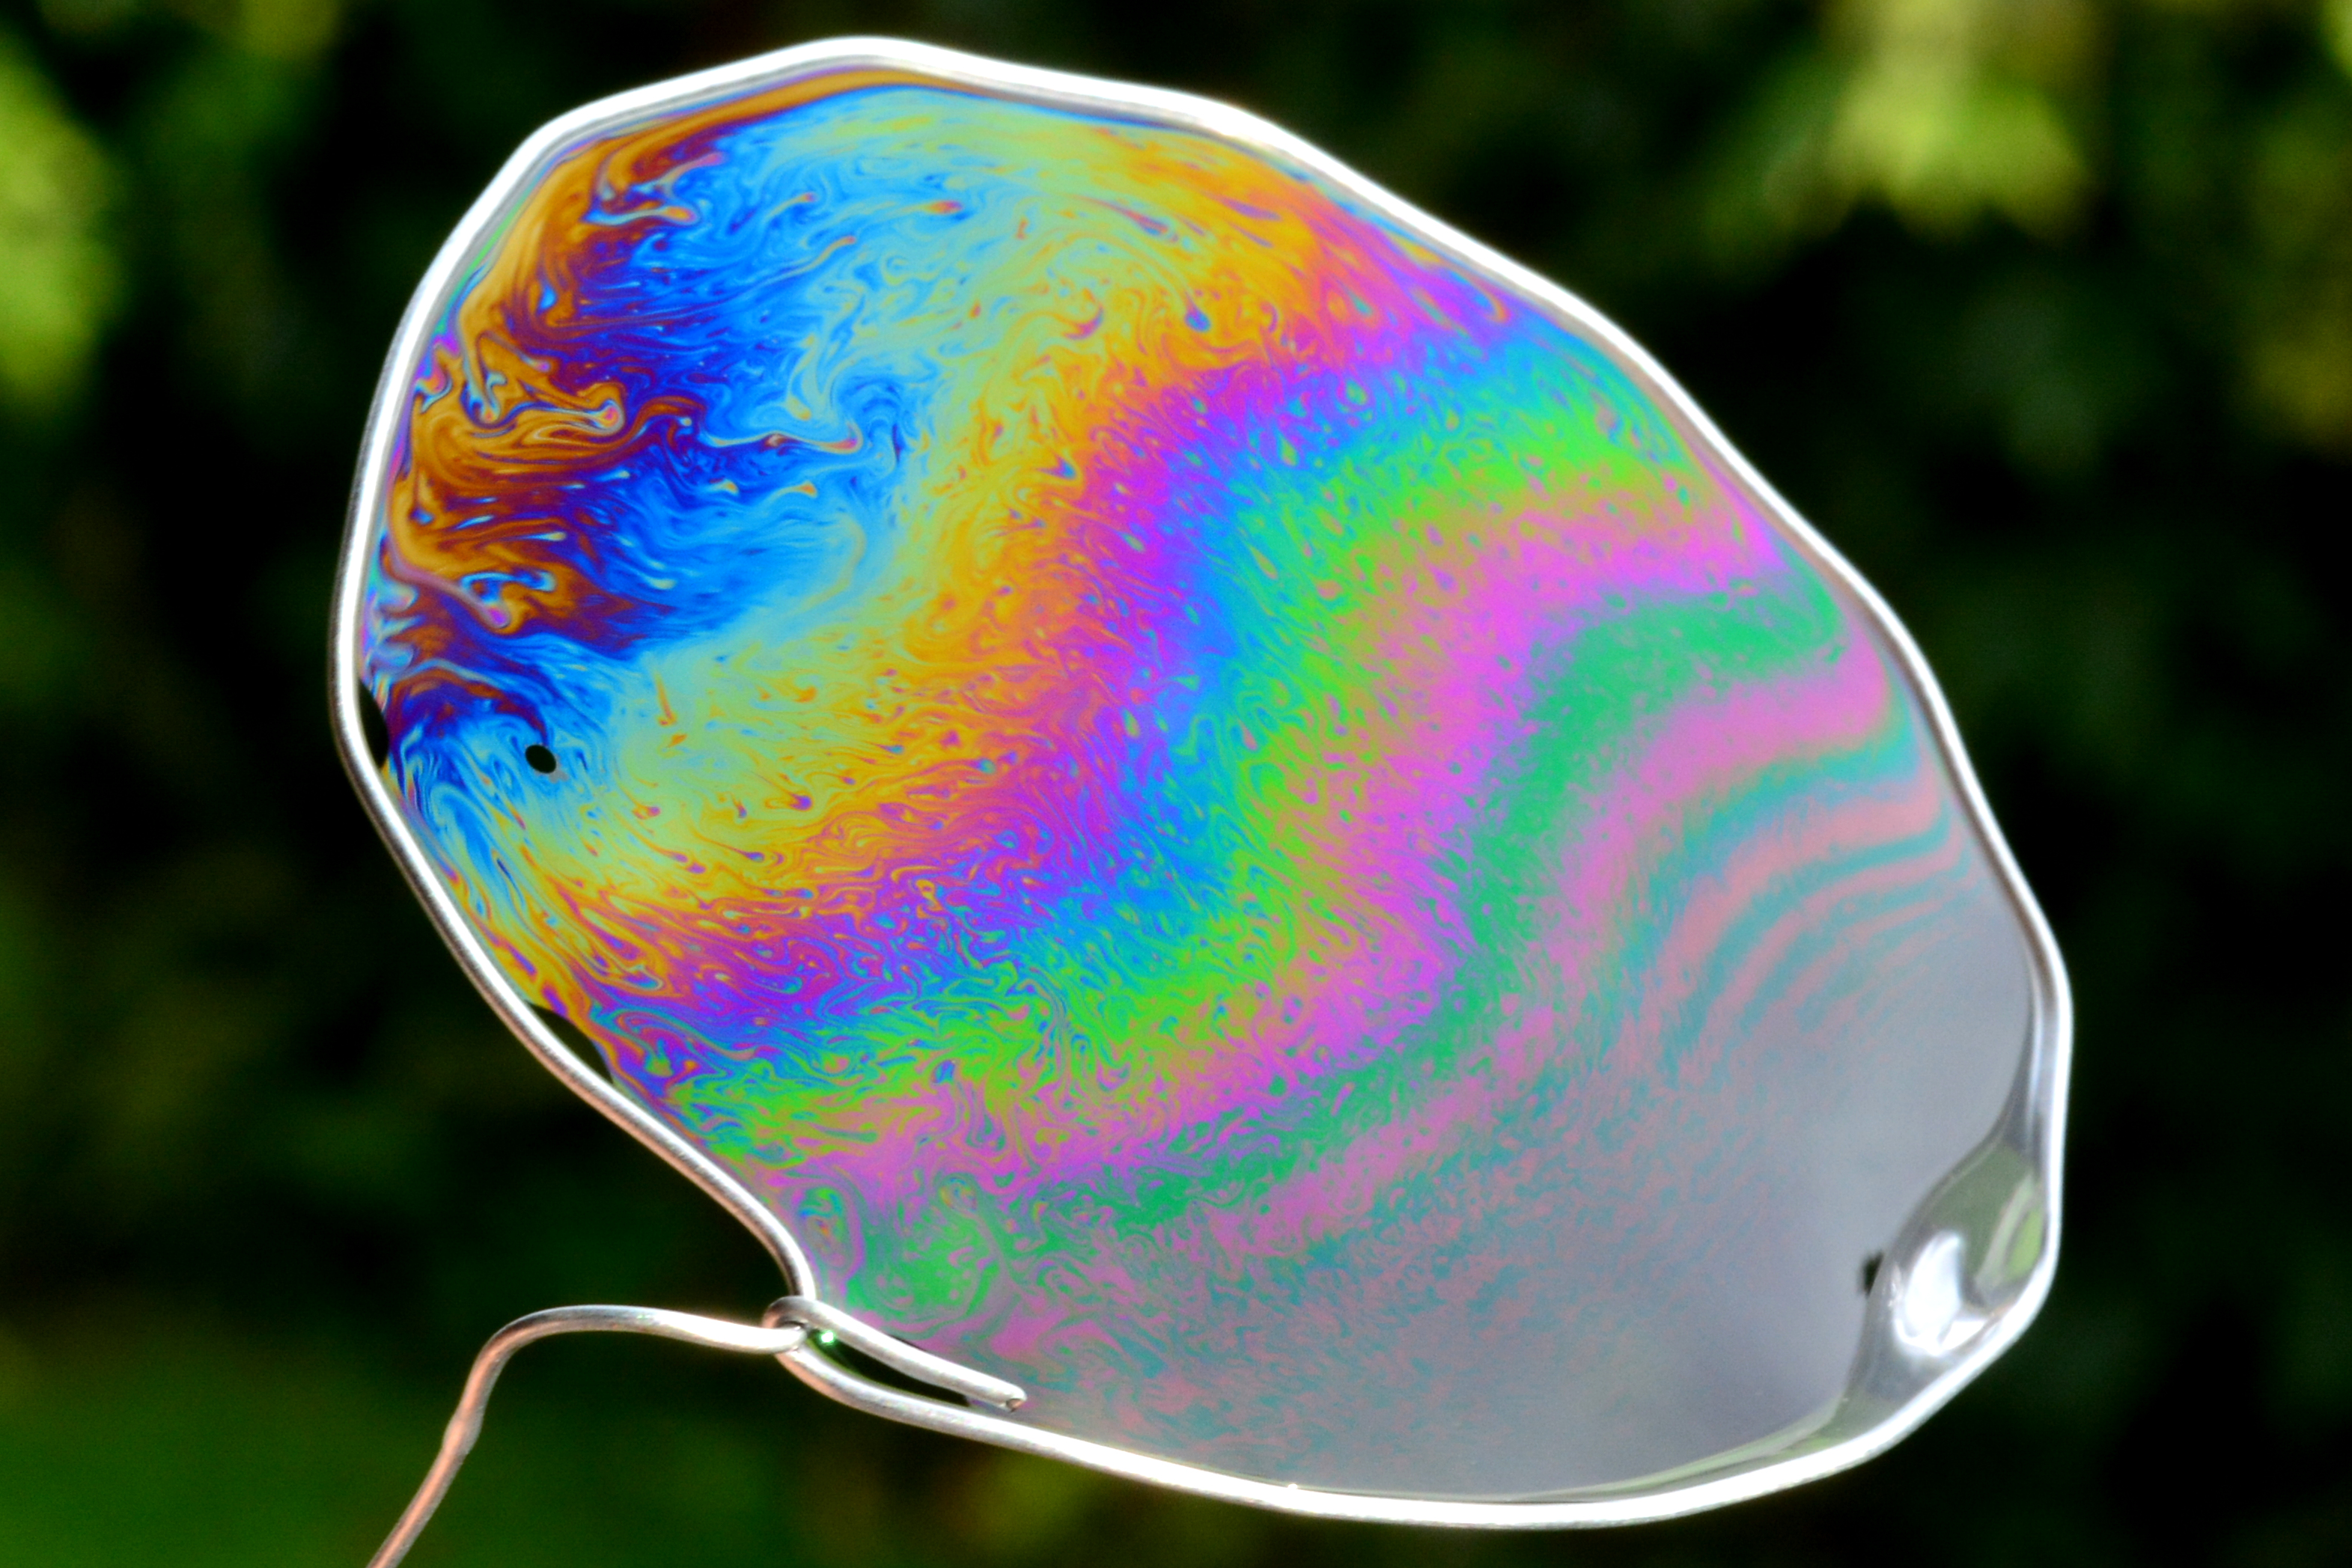
\includegraphics[width=7truecm]{slike/06_photo_soap.jpg}\newline

\includegraphics[width=7truecm]{slike/06_photo_zrak.jpg}\hfill
\includegraphics[width=7truecm]{slike/06_photo_us.jpg}
\caption{Interferenca na tanki plasti olja na vodi, milnice v zraku, tanke plasti 
zraka med objektnima stekelcema v beli in rdeči svetlobi ter interferenca
na krilih žuželke. Foto listne uši: Miran Pflaum. 
ZAMENJAJ FOTKO!!!}
\vglue-8truemm
\label{fig:06_Photos}
\end{figure}

\end{example}

\section{Večkratni odboj na tanki plasti}
Spoznali smo interferenco na tanki plasti, pri čemer
smo upoštevali le delni valovanji, ki sta se odbili na zgornji in 
spodnji meji tanke plasti. Odboje višjih redov smo zanemarili.

Zdaj se osredotočimo na interferenco velikega števila delnih 
valovanj, ki nastanejo z delitvijo amplitude na tanki plasti dielektrika.
Naj tako kot v prejšnjem razdelku ravno valovanje vpada na tanko plast 
snovi z lomnim količnikom $n_2$, lomni količnik okolice pa naj bo enak $n_1$. 
Ponovno se omejimo na primer TE polariziranega valovanja, pri katerem
je smer jakosti električnega polja pravokotna na vpadno ravnino 
(slika~\ref{fig:06_plast}). Ob vpadu na mejo med snovema se del 
svetlobe odbije, del pa lomi po lomnem zakonu (enačba~\ref{eq:lomnizakon}).
Za razliko od prej bomo zdaj upoštevali vsoto vseh prepuščenih valov, 
ki prehajajo skozi tanko plast, z ustrezno zmanjšano amplitudo.
\begin{figure}[ht]
\centering
\def\svgwidth{70truemm} 
\input{slike/06_plastmulti.pdf_tex}
\caption{Prehod svetlobe skozi tanko plast dielektrika. Delni žarki, ki prehajajo
skozi plast, med seboj interferirajo, zato je intenziteta prepuščene svetlobe odvisna
od debeline plasti $d$, lomnih količnikov plasti $n_2$ in okolice $n_1$ ter vpadnega 
kota $\alpha$. }
\vglue-2truemm
\label{fig:06_plastmulti}
\end{figure}

Zanima nas gostota prepuščenega svetlobnega toka $j$ v odvisnosti od 
lomnih količnikov $n_1$ in $n_2$, vpadnega kota $\alpha$ in debeline plasti $d$ pri dani
vpadni gostoti toka $j_0$. Spomnimo se, da za TE polarizirano valovanje
amplitudno prepustnost zapišemo z enačbo~(\ref{eq:TEr}), amplitudno odbojnost
pa z enačbo~(\ref{eq:TEt}). Ob vstopu v tanko plast tako velja:
\beq
r_{12} = \frac{n_1\cos \alpha - n_2\cos \beta}{n_1\cos \alpha + n_2\cos \beta}\qquad 
\mathrm{in}\qquad t_{12} = 1+r_{12},
\label{eq:06_35}
\eeq
ob izstopu valovanja iz tanke plasti pa:
\beq
r_{21} = \frac{n_2\cos \beta - n_1\cos \alpha}{n_2\cos \beta + n_1\cos \alpha}\qquad 
\mathrm{in}\qquad t_{21} = 1+r_{21},
\label{eq:06_36}
\eeq
pri čemer smo upoštevali, da je izhodni kot enak vpadnemu kotu $\alpha$. 

Posamezne prispevke jakosti 
električnega polja na prepuščeni strani zapišemo kot:
\begin{align}
E_1 &= E_0\,t_{12}\,t_{21},\\
E_2 &= E_0\,t_{12}\left(r_{21}\,r_{21}\,e^{i\phi}\right)t_{21},\\
E_3 &= E_0\,t_{12}\left(r_{21}\,r_{21}\,e^{i\phi}\right)
\left(\,r_{21}\,r_{21}\,e^{i\phi}\right)t_{21},\\
&...\nonumber\\
E_{N+1} &= E_0t_{12}\,\left(r_{21}\,r_{21}\,e^{i\phi}\right)^Nt_{21}.
\label{eq:06_37}
\end{align}
Upoštevali smo tudi fazni zamik med dvema sosednjima izhodnima valovanjema, do katerega
pride zaradi razlike v prepotovani poti (enačba~\ref{eq:06_34}):
\beq
\phi = 2k_0 n_2 d \cos \beta.
\label{eq:06_38}
\eeq
Celotno prepuščeno polje $E_t$ zapišemo kot vsoto vseh prispevkov (enačba~\ref{eq:06_37}) 
in dobimo:
\begin{align}
E_t &= E_1+E_2+E_3+... \nonumber \\
&= E_0\, t_{12}\,t_{21}\,\left(1 + r_{21}^2 e^{i\phi} + r_{21}^4 e^{2i\phi} 
+ r_{21}^6 e^{3i\phi} + ... \right)\!\!.
\label{eq:06_39}
\end{align}
Geometrijsko vrsto v oklepaju seštejemo in za jakost prepuščenega polja dobimo:
\beq
E_t = E_0 t= E_0 t_{12}t_{21}\frac{1}{1-r_{21}^2e^{i\phi}},
\label{eq:06_40}
\eeq
pri čemer smo vpeljali $t$ kot amplitudno prepustnost plasti. Ker sta lomni 
količnik snovi in smer širjenja svetlobe na izhodni strani enaka kot na vpadni, je 
prepustnost $T$, ki označuje razmerje med gostoto prepuščenega in vpadnega svetlobnega
toka, kar enaka $|t|^2$:
\beq
T = \frac{j}{j_0} = |t|^2= \frac{t_{12}^2t_{21}^2}{\left(1-r_{21}^2e^{i\phi}\right)
\left(1-r_{21}^2e^{-i\phi}\right)}.
\label{eq:06_41}
\eeq
Upoštevali smo, da je tanka plast dielektrična in so zato vrednosti amplitudnih 
prepustnosti in odbojnosti realne. Zapišemo še odbojnost $R = r_{21}^2$ in upoštevamo
zveze med amplitudnimi prepustnostmi in odbojnostmi:
$t_{21} = 1+r_{21}$ in $t_{12} = 1+r_{12} = 1-r_{21}$. Dobimo:
\beq
T = \frac{\left(1-R\right)^2}{1 + R^2 - 2R\cos \phi}.
\label{eq:06_42}
\eeq
Imenovalec preoblikujemo, tako da upoštevamo zvezo $\cos(2x) = 1-2\sin^2x$:
\beq
1 + R^2 - 2R\cos \phi = 1+R^2 - 2R(1-2\sin^2(\phi/2) = (1-R)^2 + 4R \sin^2(\phi/2).
\label{eq:06_43}
\eeq
Preoblikovan izraz vstavimo v enačbo~(\ref{eq:06_42}), jo delimo s števcem in 
dobimo končen izraz za prepustnost tanke plasti:
\boxeq{eq:FP}{
T = \frac{1}{1 + \frac{4R}{\left(1-R^2\right)} \sin^2(\phi/2)}.
}
Spomnimo, da je $R = r_{21}^2$ podan z enačbo~(\ref{eq:06_36}), $\phi$ pa z 
enačbo~(\ref{eq:06_38}). Izračunano odvisnost $T(\phi)$ imenujemo tudi Airyjeva 
funkcija\footnote{Ločiti je treba Airyjevo funkcijo za prepustnost 
na tanki plasti (enačba~\ref{eq:FP}) od Airyjeve funkcije v matematiki in tudi 
od Airyjevega diska, ki smo ga vpeljali pri uklonu na okrogli odprtini 
(enačba~\ref{eq:uklonAiry}.}







\section{Fabry-Perotov interferometer}

\section{Večplastni nanosi}
